\chapter{ 相关均衡}
\label{ch12:chap12}

在最后一章，我们将介绍一种新的均衡概念----\textit{相关均衡}，它比纳什均衡更具一般性。它允许参与人根据一个他们可以(通常以不同的方式)观察到的外部信号(如交通信号灯)采取随机行动，从而使他们的行动能够相互关联。

一个博弈的纳什均衡集是一组不动点，通常是不连通的。相关均衡集的范围更大，并且在数学上更简单，因为它是一个凸有界多面体。在第 12.4 节中，我们还将解释粗糙相关均衡的概念，在这种情况下，参与人承诺让相关机制为他们选择行动，而不仅仅是给他们提供建议。这一设定会限制参与人的偏离可能，进而得到一个范围更大的均衡集（该均衡集或包含更优的博弈结果，详见习题~\ref{exer:12.3}）。

因为相关均衡的集合构成一个凸多面体，所以不借助不动点定理证明其非空性将会更加简洁。事实上，Hart and Schmeidler(1989)基于极小极大定理(定理~\ref{theo:8.4})给出了这样的一个存在性证明。我们将在第 12.5 节中介绍这个证明(这一证明在这种水平的教科书中通常是找不到的)。极小极大定理为马尔可夫链平稳分布的存在性(定理~\ref{theo:12.9})和相关均衡的存在性(定理~\ref{theo:12.11})都提供了优雅的证明。

在博弈分析中，相关均衡的使用频率远低于纳什均衡，但它在博弈学习模型中有着重要作用，详见第 12.6 节列出的文献。

\section{预备知识和学习目标}


除了第 3 章中策略形式和均衡的基本概念外，主要的预备知识是第 8 章中的极小极大定理(定理~\ref{theo:8.4})。

学习本章后，你应该能够:

\begin{itemize}
\item 阐释相关均衡的定义，说明其与纳什均衡的区别，并论证相关均衡并非仅是对纳什均衡的随机化拓展。
\end{itemize}

\begin{itemize}
\item 写出定义相关均衡集的博弈的激励约束；
\end{itemize}

\begin{itemize}
\item 求解一些小博弈的激励约束，如练习~\ref{exer:12.1}；
\end{itemize}

\begin{itemize}
\item 描述粗糙相关均衡的概念以及为什么它需要参与人做出承诺；
\end{itemize}

\begin{itemize}
\item 借助极小极大定理概述相关均衡存在性的数学证明，并说明为何这一方法总体上比通过证明纳什均衡存在更为简便；
\end{itemize}

\begin{itemize}
\item 进一步详细阐述 12.5 节末尾所介绍的该存在性证明的核心思想：包括构造含关联方COR 与偏离方DEV 的辅助零和博弈，以及关联方 COR 如何抵消偏离方 DEV 的任意偏离策略。
\end{itemize}


\section{相关均衡若干示例}


上世纪末，我去耶路撒冷希伯来大学访问。在教师俱乐部里，我遇到了博弈论学者罗伯特·奥曼(Robert Aumann)和迈克尔·马施勒(Michael Maschler)。奥曼讲述了“与马施勒教授的一次交谈”如何使他产生了相关均衡的想法。他说，他们讨论了在实践中如何采用混合策略:让某个随机事件的结果决定你采取的行动。例如，如果出太阳就选择A，如果不出太阳就选择B。从天气预报中大致可以知道这种概率。但这种方法揭示了一种新的可能性:利用天气进行随机化并不会产生冯·诺伊曼(von Neumann)或纳什(Nash)所考虑的混合策略，在他们的理论中，参与人通过自己抛硬币来随机行动。如果参与人让自己的行动由天气决定，那么他们的随机选择将不是相互独立的。Aumann (1974)提出的相关均衡概念允许参与人之间采取相关的随机行动，并推广了纳什均衡的概念。(在本章中，我们始终使用“纳什均衡”这一术语来将其与其他均衡概念区分开来。)本章的主题就是相关均衡。

考虑图~\ref{fig:12.1}中胆小鬼博弈的变形。每个参与人有两个策略，这里参与人I的策略命名为 \(T\) 和 \(B\) ，参与人II的策略命名为 \(L\) 和 \(R\) 。与图~\ref{fig:3.3}中的原始胆小鬼博弈相比，如果另一个参与人采用她的第二种策略，那么该参与人的收益会增加3 (根据命题~\ref{prop:9.7}，或者直接观察可知，这并不影响对任何混合策略的最优反应)。该博弈有两个非对称的纯纳什均衡:(B，L)，参与人 \(\mathrm{I}\) 和 \(\mathrm{{II}}\) 的收益分别为1和5；以及(T，R)，收益分别为5和1。在唯一的混合均衡中，两个参与人都采用混合策略 \(\left( {\frac{1}{2},\frac{1}{2}}\right)\) ，每个参与人的收益为 \(\frac{5}{2}\) 。

\begin{figure}[htbp]
\centering
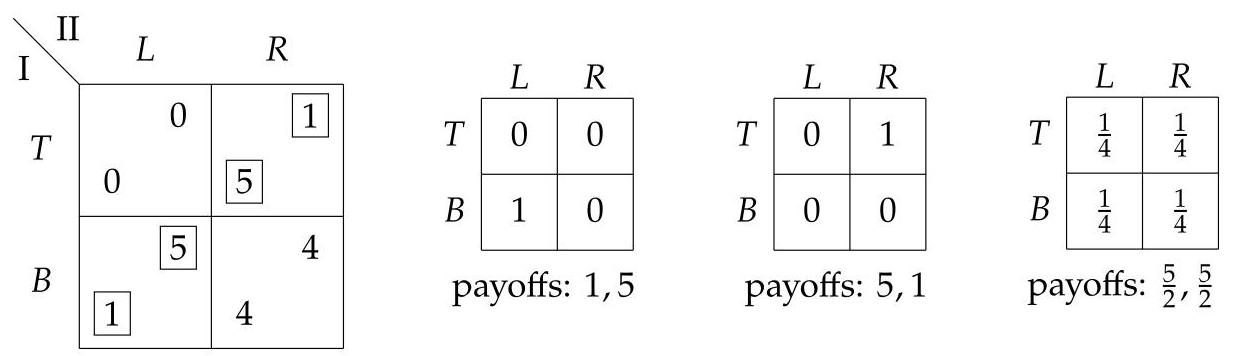
\includegraphics[width=0.9\textwidth]{images/ch12-fig01.jpg}
\caption{图~\ref{fig:3.3}中胆小鬼博弈的一个变形。右侧的三个表格展示了该博弈的三个纳什均衡对应的策略组合的概率分布。}
\label{fig:12.1}
\end{figure}

图~\ref{fig:12.1}右侧的三个面板展示了该博弈的三个纳什均衡对应的四个策略对的概率分布。纯纳什均衡只选择一个策略对。混合纳什均衡以相等的概率 \(\frac{1}{4}\) 选择每个策略对。

在相关均衡中，这种概率分布被视为一种相关机制，它随机选择一个纯策略组合，并将该组合中每个参与人的策略私下告知该参与人，作为对其行动的建议。假设每个参与人都知道该机制的运作方式，并且可以从自己得到的建议推断出其他参与人得到的建议。则均衡条件是，假设其他参与人遵循他们的建议，那么每个参与人选择被建议的行动是最优的。


对于图~\ref{fig:12.1}中的第一个纯纳什均衡(B，L)，该机制选择这个策略对，并建议参与人I采用 \(B\) ，参与人II采用 \(L\) 。在这里，每个参与人都知道对方得到的建议，并且知道自己得到的建议是对对方策略的最优反应，因此这是一个相关均衡。这同样适用于第二个纯均衡(T，R)。

在图~\ref{fig:12.1}中的第三个混合纳什均衡中，该机制以相等的概率选择每个策略对。这包括本身并非纳什均衡的策略对，例如(T，L)。如果该机制选择(T，L)，那么参与人 \(\mathrm{I}\) 被建议采用 \(T\) 。然而，关键的是，参与人 \(\mathrm{I}\) 并不知道参与人II被建议采用L。参与人I只能从自己被建议采用 \(T\) 这一事实推断出参与人II被建议采用 \(L\) 和 \(R\) 的概率相等(当参与人 \(\mathrm{I}\) 被建议采用 \(B\) 时也是如此)。鉴于参与人II的这种随机选择，自己的两个策略对于参与人I来说无差异，因此遵循被建议的行动是最优的。对于该机制选择的任何策略对都是如此。因此，它也是一个相关均衡。

\begin{figure}[htbp]
\centering
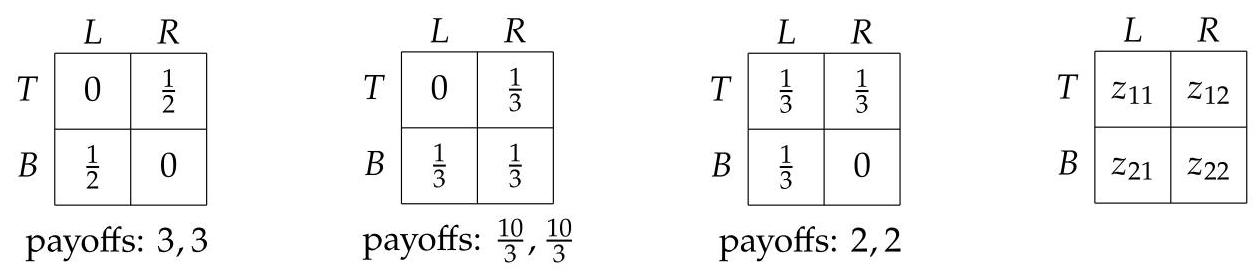
\includegraphics[width=0.9\textwidth]{images/ch12-fig02.jpg}
\caption{展示了图~\ref{fig:12.1}中博弈的相关均衡示例及其期望效用。右侧显示了相关分布的一般形式。}
\label{fig:12.2}
\end{figure}


在双矩阵博弈的混合纳什均衡(x, y)中，由于两个参与人独立地进行随机化选择，纯策略对(i, j)被选中的概率为 \({x}_{i}{y}_{j}\) 。在双矩阵博弈的相关均衡中，每个策略对 (i, j) 都有一定的概率 \({z}_{ij}\) ，称为该策略对的联合概率。图~\ref{fig:12.2}展示了更一般的此类概率分布。在左图中，两个策略对 (B, L) 和 (T, {\color{blue}R}) 被选中的概率相等。无论选择哪一对，两个参与人都能确定地知道对另一个参与人的建议。这两个纯策略互为最优反应，因此均衡条件成立。在这里，装置选择另外两个策略对 (T, L) 和 (B, R) 的概率为零。联合概率分布不是独立的，而是相关的，也就是说，它不能表示为 \({z}_{ij} = {x}_{i}{y}_{j}\) 的形式，因为，例如， \({z}_{11} = 0\) 意味着 \({x}_{1} = 0\) 或 \({y}_{1} = 0\) ，其中 \({x}_{1} = 0\) 意味着 \({z}_{12} = 0\) ， \({y}_{1} = 0\) 意味着 \({z}_{21} = 0\) ，但 \({z}_{12}\) 和 \({z}_{21}\) 都是正数。

图~\ref{fig:12.2}左图中的这个相关均衡为每个参与人提供了3的期望效用，这在任何纳什均衡中都无法实现。作为纯纳什均衡之间的平等“混合”，它似乎也是一种公平的博弈方式。这可以通过抛一枚公平的硬币来实现，硬币的结果决定了应该采用哪一个纯纳什均衡。


然而，通过图~\ref{fig:12.2}第二图所示的装置，参与人可以获得更高的期望效用。在那里，每个参与人收益为3的策略对 (B, R) 的概率为 \(\frac{1}{3}\) ，与另外两个策略对 (B, L) 和 (T, R) 相同。左上角收益为0,0的策略对 (T, L) 的概率为零。如果装置选择 (B, R)，那么参与人I(参与人II同理)只知道另一个参与人被建议采用任一纯策略的概率为 \(\frac{1}{2}\) ，对此策略{\color{blue}B}是最优反应。如果装置选择 (B, L)，那么参与人I也能推断出参与人II被建议以概率 \(\frac{1}{2}\) 采用任一策略，而参与人II知道参与人I肯定被建议采用策略{\color{blue}B}；反之，当装置选择 (T, L) 时情况相同。因此，这也是一个相关均衡，期望效用为 \(\left( {\frac{10}{3},\frac{10}{3}}\right)\) 。可以证明，这个相关均衡使两个参与人的期望效用之和最大。

然而，也可能存在相关均衡，其期望效用比任何纳什均衡都差，如图~\ref{fig:12.2}第三图所示。在那里，装置以概率 \(\frac{1}{3}\) 选择收益较差的策略对 (T, L)(收益为0,0)，而以概率零选择收益较好的策略对 (B, R)(收益为4,4)。出于与之前相同的原因，这是一个相关均衡:每个参与人从自己得到的建议中推断出对手是确定性选择还是以 \(\left( {\frac{1}{2},\frac{1}{2}}\right)\) 的概率随机选择，而自己得到的建议对此是最优反应。然而，每个参与人的期望效用为 \(\frac{0 + 5 + 1}{3} = 2\) ，该均衡下参与人收益之和比任何纳什均衡都差。

\section{激励约束}

本节将对相关均衡的概念进行形式化定义，为简化符号表达，首先针对双人博弈展开分析。考虑一个 \(m\times n\) 双矩阵博弈 \((A,B)\) ，如果参与人 I 和参与人 II 分别选择第 \(i\) 行和第 \(j\) 列，他们的收益分别为 \(a_{ij}\) 和 \(b_{ij}\) 。相关机制(correlation device)是纯策略对的一个概率分布 \(z\) ，策略对 \((i,j)\) 的概率为 \(z_{ij}\) ，其中这些数值满足；

\begin{equation}
{z}_{ij} \geq  0\;\left( {1 \leq  i \leq  m,1 \leq  j \leq  n}\right) ,\;\mathop{\sum }\limits_{{i = 1}}^{m}\mathop{\sum }\limits_{{j = 1}}^{n}{z}_{ij} = 1. \label{eq:12.1}
\end{equation}

这些概率是参与人的共同知识。该机制根据这些概率选择一个策略对，并私下只告知每个参与人他在该策略对中的纯策略。假设参与人 I 被告知选择策略 \(i\) 。那么，该机制的第 \(i\) 行(如图~\ref{fig:12.2} 中的各子图所示)给出了参与人 II 被告知选择各列 \(j\) 的概率 \(p_{ij}\) 。已知参与人 I 被告知选择 \(i\) ，那么参与人 II 选择第 \(j\) 列的条件概率为；

\begin{equation}
\operatorname{prob}\left( {j \mid  i}\right)  = \frac{{z}_{ij}}{\mathop{\sum }\limits_{{l = 1}}^{n}{z}_{il}}. \label{eq:12.2}
\end{equation}

只要 \(p\) 以正概率选择第 \(i\) 行，这个表达式就是有定义的，因为此时至少存在一个列 \(j\) 使得 \(p_{ij}>0\) ，从而\eqref{eq:12.2}式中的分母为正。这个条件概率分布就是参与人 I(当被告知选择第 \(i\) 行时)对参与人 II 被推荐采取的行动 \(j\) 的推断。如果参与人 I 遵循被推荐的行动 \(i\) ，他将获得一定的期望效用。在参与人 II 随机选择 \(j\) 的相同条件分布下，如果没有其他行 \(i'\) 能给参与人 I 带来更高的期望效用(因为当参与人 I 从 \(i\) 偏离到 \(i'\) 时，他不会获得更多信息)，那么这个收益对参与人 I 来说就是最优的。也就是说，对于所有其他行 \(i'\) ，我们要求

\begin{equation}
\mathop{\sum }\limits_{{j = 1}}^{n}{a}_{ij}\frac{{z}_{ij}}{\mathop{\sum }\limits_{{l = 1}}^{n}{z}_{il}} \geq  \mathop{\sum }\limits_{{j = 1}}^{n}{a}_{kj}\frac{{z}_{ij}}{\mathop{\sum }\limits_{{l = 1}}^{n}{z}_{il}}. \label{eq:12.3}
\end{equation}


两边同时乘以 \(\mathop{\sum }\limits_{{l = 1}}^{n}{z}_{il}\) 表明\eqref{eq:12.3}式等价于

\begin{equation}
\mathop{\sum }\limits_{{j = 1}}^{n}\left( {{a}_{ij} - {a}_{kj}}\right) {z}_{ij} \geq  0\;\left( {1 \leq  i,k \leq  m}\right) . \label{eq:12.4}
\end{equation}

对于式 \eqref{eq:12.4} 中所有数对 $i,k$ 对应的 $m^2$ 个不等式：当 $i = k$ 时，该不等式显然成立；当 $\sum\limits_{l=1}^{n} z_{il} = 0$（即在行分布 $z$ 下第 $i$ 行的概率为 0）时，该不等式也显然成立——因为这意味着对于该 $i$ 行，所有 $j$ 均满足 $z_{ij} = 0$。若 $\sum\limits_{l=1}^{n} z_{il} > 0$，则式 \eqref{eq:12.4} 可推导出式 \eqref{eq:12.3}，且表明参与人 I 没有动机从推荐的第 $i$ 行偏离至第 $k$ 行。因此，不等式 \eqref{eq:12.4} 被称为参与人 I 的激励约束。参与人 II 对应的激励约束为：

\begin{equation}
\mathop{\sum }\limits_{{i = 1}}^{m}\left( {{b}_{ij} - {b}_{il}}\right) {z}_{ij} \geq  0\;\left( {1 \leq  j,l \leq  n}\right)  \label{eq:12.5}
\end{equation}

该式表明，当参与人 II 被推荐选择第 \(j\) 列时，他没有动机偏离到第 \(j'\) 列。

\begin{definition}[两个参与人的相关均衡]\label{def:12.1}
对于一个 \(m \times n\) 的双矩阵博弈 \((A, B)\)，相关均衡是一个 \(m \times n\) 的矩阵 \(z\)，其元素为策略对 \((i, j)\) 的联合概率。该矩阵需满足式 \eqref{eq:12.1}，以及参与人 I 的激励约束 \eqref{eq:12.4} 和参与人 II 的激励约束 \eqref{eq:12.5}。矩阵 \(z\) 定义了一个相关装置：它以概率 \(z_{ij}\) 选择策略对 \((i, j)\)，然后分别私下告知参与人 I 选择策略 \(i\)、参与人 II 选择策略 \(j\)（不向对方透露信息）。
\end{definition}
玩家 \(\mathrm{I}\) 的激励约束 \eqref{eq:12.4} 是针对矩阵 \(z\) 的每一行 \(i\) 的。通过归一化（如公式 \eqref{eq:12.3} 所示），该行 \(z\) 表示玩家 I 在被推荐选择 \(i\) 后对玩家 II 行为的“后验”判断。这可以看作是对玩家 II 的一种推断的“混合策略”，在该混合策略下，第 \(i\) 行是最优反应；一般而言，这种推断的混合策略依赖于 \(i\)。同样地，玩家 II 的激励约束 \eqref{eq:12.5} 是针对矩阵 \(z\) 的每一列 \(j\) 的，其描述（经过归一化）了对玩家 I 的推断混合策略，在该混合策略下，第 \(j\) 列是最优反应。如果 \(z\) 是通过纳什均衡得到的，即 \({z}_{ij} = {x}_{i}{y}_{j}\)，那么对手推断出来的这些混合策略始终相同，即实际的混合策略。

\begin{proposition}\label{prop:12.2}
设 (A, B) 是一个 \(m \times  n\) 双矩阵博弈，设 \(x\) 是参与人 \(I\) 的一个混合策略， \(y\) 是参与人 \({II}\) 的一个混合策略，并且对于所有的 \(i\) 和 \(j\) ，定义 \(z \in  {\mathbb{R}}^{m \times  n}\) 满足\({z}_{ij} = {x}_{i}{y}_{j}\) 。则 \(z\) 是 (A, B) 的一个相关均衡，当且仅当 (x, y) 是 (A, B) 的一个纳什均衡。
\end{proposition}

\begin{proof}
显然， \(\mathop{\sum }\limits_{{i = 1}}^{m}{x}_{i} = 1\) 和 \(\mathop{\sum }\limits_{{j = 1}}^{n}{y}_{j} = 1\) 意味着 \(z\) 是如\eqref{eq:12.1}中所述的关于对 (i, j) 的一个概率分布。因为 \(\mathop{\sum }\limits_{{l = 1}}^{n}{y}_{l} = 1\) 和 \({z}_{il} = {x}_{i}{y}_{l}\) ，我们有对于 \(1 \leq  i \leq  m\) 的 \(\mathop{\sum }\limits_{{l = 1}}^{n}{z}_{il} = {x}_{i}\) 。

假设 \(z\) 是一个相关均衡。如果 \({x}_{i} > 0\) ，那么\eqref{eq:12.4}蕴含着\eqref{eq:12.3}，即 \(\mathop{\sum }\limits_{{j = 1}}{a}_{ij}{y}_{j} \geq  \mathop{\sum }\limits_{{j = 1}}{a}_{kj}{y}_{j}\) ，也就是说，参与人 \(\mathrm{I}\) 在 \(i\) 行的期望效用至少和在任何其他行 \(k\) 的一样大。根据最优反应条件\eqref{eq:6.11}，这意味着 \(x\) 是对 \(y\) 的最优反应。类似地，\eqref{eq:12.5}意味着 \(y\) 是对 \(x\) 的最优反应。因此，(x, y) 是一个纳什均衡。

如果 (x, y) 是一个纳什均衡，这些蕴含关系反过来也成立:如果 \({x}_{i} = 0\) ，\eqref{eq:12.4}显然成立，并且如果 \({x}_{i} > 0\) ， \(i\) 行的期望效用至少是任何其他行 \(k\) 的期望效用。这一事实意味着\eqref{eq:12.3}，从而意味着\eqref{eq:12.4}。类似地， \(y\) 是对 \(x\) 的最优反应等价于\eqref{eq:12.5}。因此，两个参与人的激励约束都成立，故 \(z\) 是一个相关均衡。
\end{proof}

激励约束\eqref{eq:12.4}和\eqref{eq:12.5}分别涉及两个收益矩阵 \(A\) 和 \(B\) ，但共同影响矩阵 \(z\) 。\eqref{eq:12.4}中有 \(m\left( {m - 1}\right)\) 个非平凡约束(对于 \(i = k\) 它们是平凡的)，\eqref{eq:12.5}中有 \(n\left( {n - 1}\right)\) 个非平凡约束。对于图~\ref{fig:12.1} 中的博弈，它们表述为

\begin{equation}
- {z}_{11} + {z}_{12} \geq  0,\;{z}_{21} - {z}_{22} \geq  0, \label{eq:12.6}
\end{equation}

\[
- {z}_{11} + {z}_{21} \geq  0,\;{z}_{12} - {z}_{22} \geq  0,
\]

也就是说， \({z}_{12}\) 和 \({z}_{21}\) 都必须至少与 \({z}_{11}\) 和 \({z}_{22}\) 一样大。如 \eqref{eq:12.1} 所示，纯策略对的所有联合分布 \(z\) 的集合是一个维度为 \({mn} - 1\) 的单纯形，这里是一个三维的四面体。额外的激励约束 \eqref{eq:12.4} 和 \eqref{eq:12.5} 定义了所有相关均衡的集合。相关均衡的集合是该单纯形的一个子集，且是一个有界多面体。

对于我们具有激励约束 \eqref{eq:12.6} 的 \(2 \times  2\) 博弈，该有界多面体如图~\ref{fig:12.3} 所示。它有五个顶点，包括 \(\left( {{z}_{11},{z}_{12},{z}_{21},{z}_{22}}\right)  = \left( {0,0,1,0}\right) ,\left( {0,1,0,0}\right)\) 和 \(\left( {\frac{1}{4},\frac{1}{4},\frac{1}{4},\frac{1}{4}}\right)\) 。这些是图~\ref{fig:12.1} 中的纯纳什均衡和混合纳什均衡，在图~\ref{fig:12.3} 中标记为 \({BL},{TR}\) 和 \(M\) 。相关均衡集的另外两个顶点是 \(\left( {0,\frac{1}{3},\frac{1}{3},\frac{1}{3}}\right)\) 和 \(\left( {\frac{1}{3},\frac{1}{3},\frac{1}{3},0}\right)\) 。图~\ref{fig:12.2} 中的两个中间图片展示了这两个顶点(其左图 \(\left( {0,\frac{1}{2},\frac{1}{2},0}\right)\) 是 (0,0,1,0) 和 (0,1,0,0) 的凸组合，不是顶点)。任意一个这样的顶点都可以通过令\eqref{eq:12.1} 和 \eqref{eq:12.6} 中的至少三个不等式成为等式得到。这些等式可以得到唯一解。

对于有 \(N\) 个参与人的博弈，相关均衡有类似的定义。回顾定义~\ref{def:3.1}，在一个 \(N\) 参与人博弈中，一个策略组合 \(s = \left( {{s}_{1},\ldots ,{s}_{N}}\right)\) 也可以写成 \(\left( {{s}_{i},{s}_{-i}}\right)\) ，其中包含参与人 \(i\) 的策略 \({s}_{i}\) 以及其余参与人的部分策略组合 \({s}_{-i}\) ，这些部分策略组合的集合是 \({S}_{-i} = { \times  }_{j = 1,j \neq  i}^{n}{S}_{j}.\)


\begin{definition}[\(N\) 人博弈的相关均衡]\label{def:12.3}
设 \(G\) 是一个 \(N\) 个参与人的策略式博弈，参与人 \(i = 1,\ldots ,N\) 拥有有限策略集 \({S}_{i}\) ，对于 \(S = {S}_{1} \times  \cdots  \times  {S}_{N}\) 中的每个策略组合 \(s = \left( {{s}_{1},\ldots ,{s}_{N}}\right)\) ，其收益为 \({u}_{i}\left( s\right)\) 。一个相关机制是策略组合上的一个概率分布 \(z\) ，即一个函数 \(z : S \rightarrow  \mathbb{R}\) ，满足

\begin{equation}
z\left( s\right)  \geq  0\;\left( {s \in  S}\right) ,\;\mathop{\sum }\limits_{{s \in  S}}z\left( s\right)  = 1. \label{eq:12.7}
\end{equation}
\end{definition}

\begin{figure}[htbp]
\centering
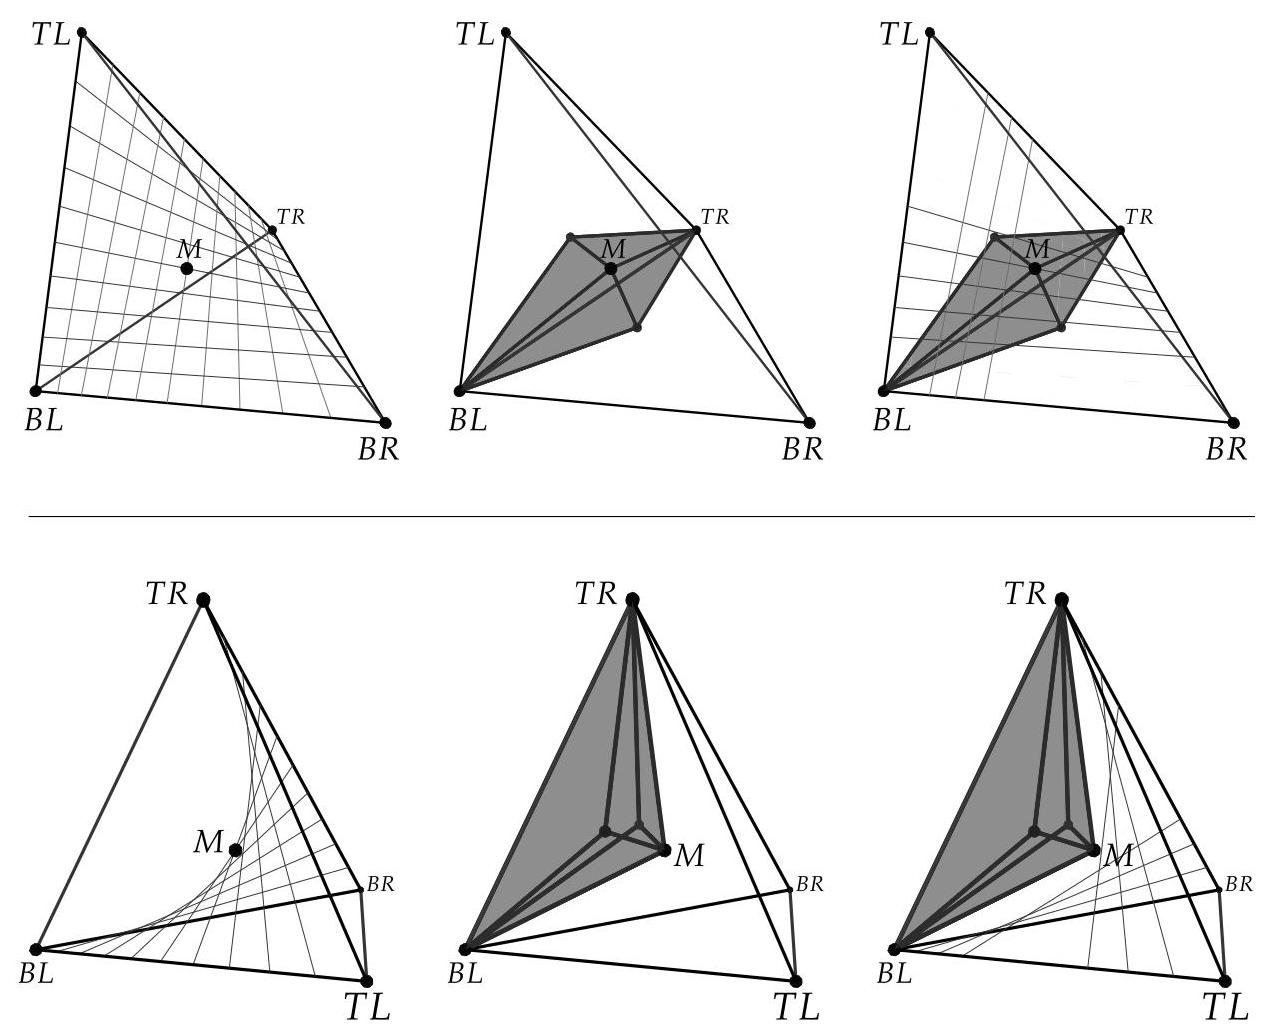
\includegraphics[width=0.9\textwidth]{images/ch12-fig03.jpg}
\caption{图~\ref{fig:12.1} 中博弈的联合分布 \(z\)的单纯形的两个视角，其中有 \({TL},{TR},{BL},{BR}\) (代表四个纯策略对)和混合纳什均衡 \(M\) 。左图显示了由 \({z}_{ij} = {x}_{i}{y}_{j}\) 定义的非相关策略，中图显示了由额外激励约束 \eqref{eq:12.6} 定义的相关均衡的有界多面体，右图同时显示了这两个集合，它们的交集定义了纳什均衡\({BL},{TR},M\) ，如命题~\ref{prop:12.2} 所述。}
\label{fig:12.3}
\end{figure}

参与人们知道 \(z\) 。相关机制以概率 \(z\left( s\right)\) 选择策略组合 \(s\) ，然后私下告知每个参与人 \(i\) 在 \(s\) 中各自的策略 \({s}_{i}\) 。如果对于每个参与人 \(i = 1,\ldots ,N\) ，激励约束:

\begin{equation}
\mathop{\sum }\limits_{{{s}_{-i} \in  {S}_{-i}}}\left( {{u}_{i}\left( {{s}_{i},{s}_{-i}}\right)  - {u}_{i}\left( {{t}_{i},{s}_{-i}}\right) }\right) z\left( {{s}_{i},{s}_{-i}}\right)  \geq  0\;\left( {{s}_{i},{t}_{i} \in  {S}_{i}}\right)  \label{eq:12.8}
\end{equation}

成立，那么 \(z\) 被称为 \(G\) 的相关均衡。

激励约束\eqref{eq:12.8}推广了两个参与人情形下\eqref{eq:12.4}和\eqref{eq:12.5}中的约束。在\eqref{eq:12.8}中，参与人 \(i\) 被要求采用策略 \({s}_{i}\) ，并能从这个信息推断出其他参与人所有可能的部分策略组合 \({s}_{-i}\) 的绝对概率 \(z\left( {{s}_{i},{s}_{-i}}\right)\) 。这些概率之和为正，因为否则参与人 \(i\) 不可能被要求采用 \({s}_{i}\) 。用这个和去除这些概率，就得到了其他参与人被要求采用的策略的条件概率，与\eqref{eq:12.3}类似，该不等式表明参与人 \(i\) 从 \({s}_{i}\) 偏离到任何其他策略 \({t}_{i}\) 都无利可图。这就是均衡性质。

命题~\ref{prop:12.2}对于 \(N\) 个参与人同样成立。

\begin{proposition}\label{prop:12.4}
考虑如定义~\ref{def:12.3}中所述的 \(N\) 人策略式博弈 \(G\) ，并为每个参与人 \(i\) 设定一个混合策略 \({\sigma }_{i}\) 。假设 \(z\) 是一个相关机制，使得对于所有 \(s = \left( {{s}_{1},\ldots ,{s}_{N}}\right)  \in  S\) 有 \(z\left( s\right)  = \mathop{\prod }\limits_{{i = 1}}^{N}{\sigma }_{i}\left( {s}_{i}\right)\) 。那么 \(z\) 是 \(G\) 的相关均衡，当且仅当 \(\left( {{\sigma }_{1},\ldots ,{\sigma }_{N}}\right)\) 是 \(G\) 的纳什均衡。
\end{proposition}

\begin{proof}
通过应用 \(N\) 个参与人的最优反应条件(见命题~\ref{prop:6.3})，命题~\ref{prop:12.2}的证明可以照搬过来。
\end{proof}

定义~\ref{def:12.3}中博弈 \(G\) 的相关均衡 \(z\) 由其策略组合的概率 \(z\left( s\right)\) 定义，使得激励约束\eqref{eq:12.8}成立。这些约束，以及表明 \(z \in  \Delta \left( S\right)\) 的条件\eqref{eq:12.7}，对于 \(s \in  S\) 的变量 \(z\left( s\right)\) 是线性的。因此， \(G\) 的相关均衡集是一个多面体，并且作为单纯形 \(\Delta \left( S\right)\) 的子集是有界的，所以是一个有界多面体。在数学上，这比 \(G\) 的纳什均衡集更简单，后者一般不是凸集。然而，到目前为止， \(N\) 人博弈 \(G\) 存在相关均衡的唯一证明是通过纳什均衡的存在性，这依赖于布劳威尔不动点定理。第12.5节将给出另一个证明：使用冯·诺伊曼极小极大定理给出相关均衡存在性的优雅证明。


\section{粗糙相关均衡}

相关均衡需要一个相关机制。例如，交通信号灯向不同的道路使用者发送相关信号，这些信号是对行动的建议。均衡条件是，假设其他参与者都会遵循这些建议，那么遵循建议对你而言就是最优选择。

在本节中，我们考虑一个更进一步的概念。相关机制不仅建议行动，而且每个参与人都承诺遵循被建议的行动(例如让该机制选择行动，就像在自动驾驶汽车中那样)。为了将其构建成一个博弈，参与人的选择发生在更早的阶段，即是否参与使用这个机制。


假设在如定义~\ref{def:12.3}中所述的博弈 \(G\) 中，相关装置是策略组合集上的一个概率分布 \(z \in  \Delta \left( S\right)\) 。如果所有参与人都参与，那么某个组合 \(s\) 将由 \(z\) 选择并被参与人使用。如果参与人 \(i\) 不参与，他只知道由 \(z\) 给出的其他参与人的部分组合 \({s}_{-i}\) 的边际概率分布。然后参与人 \(i\) 可以选择他自己的最优行动 \({s}_{i} \in  {S}_{i}\) ，但不知道该机制会选择什么行动。{\color{red}如果相对于边际分布，他参与该方案无法获得收益，并且这适用于每个参与人 \(i\) ，那么 \(z\) 就被称为粗糙相关均衡。}

\begin{figure}[htbp]
\centering
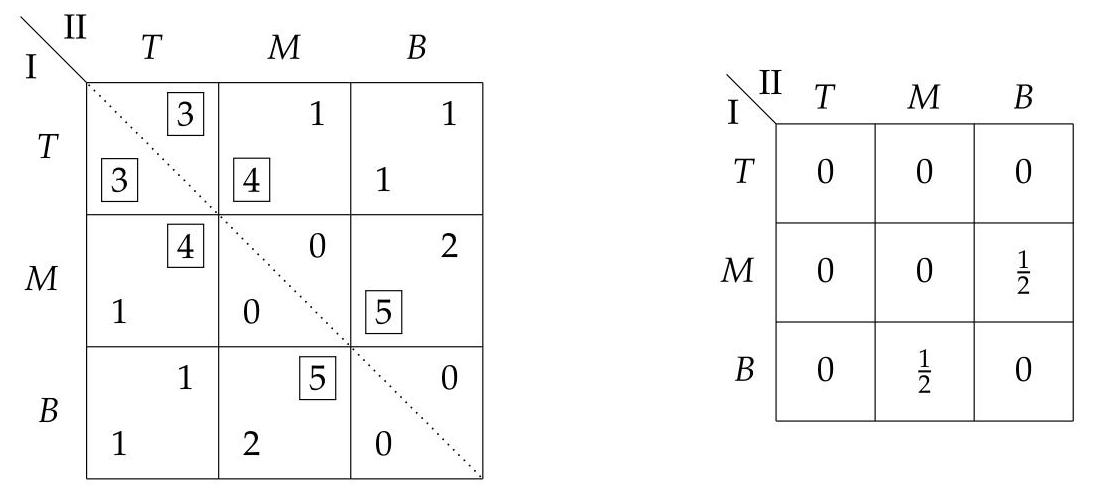
\includegraphics[width=0.8\textwidth]{images/ch12-fig04.jpg}
\caption{左:占优可解的 \(3 \times  3\) 博弈，具有唯一的纳什均衡和相关均衡(T, T)。右:策略对的分布，它是一个粗略相关均衡，其收益高于纳什均衡。}
\label{fig:12.4}
\end{figure}

图~\ref{fig:12.4}展示了一个对称的 \(3 \times  3\) 博弈的例子。该博弈是占优可解的(见命题~\ref{prop:3.4}):策略 \(B\) 被策略 \(T\) 严格占优(对两个参与人都是如此)，并且在剔除 \(B\) 之后，在剩余的 \(2 \times  2\) 博弈中，策略 \(M\) 被 \(T\) 严格占优，因此(T, T)是该博弈的唯一纳什均衡。根据以下命题，它也是唯一的相关均衡。

\begin{proposition}\label{prop:12.5}
考虑一个 \(N\) 人博弈，其中参与人 \(i\) 的纯策略 \({t}_{i}\) 严格占优他的纯策略 \({s}_{i}\) 。那么在该博弈的任何相关均衡 \(z\) 中，策略 \({s}_{i}\) 永远不会被推荐给参与人 \(i\) 。
\end{proposition}

\begin{proof}
 \({t}_{i}\) 对 \({s}_{i}\) 的严格占优在\eqref{eq:3.4}中给出，这等价于\eqref{eq:12.8}中的 \({u}_{i}\left( {{s}_{i},{s}_{-i}}\right)  - {u}_{i}\left( {{t}_{i},{s}_{-i}}\right)\) 对所有 \({s}_{-i} \in  {S}_{-i}\) 都是负的。因此，不等式\eqref{eq:12.8}只有在对所有 \({s}_{-i}\) 都有 \(z\left( {{s}_{i},{s}_{-i}}\right)  = 0\) 时才成立。这意味着 \({s}_{i}\) 永远不会是 \(z\) 选择的任何策略组合 \(s\) 的一部分，因此 \(z\) 永远不会告诉参与人 \(i\) 选择 \({s}_{i}\) 。
\end{proof}

现在考虑图~\ref{fig:12.4}右侧所示的相关机制，它以概率 \(\frac{1}{2}\) 分别选择策略组合(M, B)和(B, M)。它定义了一个粗糙相关均衡:如果每个参与人都承诺执行该机制选择的行动，那么每个参与人的期望效用是 \(\frac{7}{2}\) 。或者，参与人可以选择不使用该机制，然后，假设另一个参与人使用该机制，他只知道另一个参与人将以概率 \(\frac{1}{2}\) 分别选择 \(M\) 和 \(B\) 。选择不使用该机制的参与人在选择 \(T,M\) 或 \(B\) 时的相应收益分别是 \(\frac{5}{2},\frac{5}{2}\) 和1，这两个收益都更低，因此参与人承诺使用该机制是最优的。此外，每个参与人的收益都高于唯一的纳什均衡和相关均衡。

以下是粗糙相关均衡的正式定义

\begin{definition}\label{def:12.6}
考虑一个 \(N\) 人博弈，采用定义~\ref{def:12.3}中的符号。考虑一个参与人们都知晓的相关机制 \(z\) ，每个参与人事先都可以预先选择：或者遵循该机制从 \(z\) 选出的策略组合中分配给自己的纯策略，或者选择退出这一机制，在不知道机制选择的情况下选择任何策略。如果每个参与人都选择遵循该机制的选择，并且没有单方面偏离的动机，那么这被称为一个粗糙相关均衡。
\end{definition}

以下内容表明粗糙相关均衡比相关均衡更具一般性，并且在式\eqref{eq:12.9}中给出了刻画粗略相关均衡的约束条件。

\begin{proposition}\label{prop:12.7}
每个相关均衡都是一个粗略相关均衡。
\end{proposition}

\begin{proof}
考虑一个粗糙相关均衡 \(z\) 。如果每个参与人都承诺执行 \(z\) 所选择的行动，那么参与人 \(i\) 的期望效用是 \(\mathop{\sum }\limits_{{s \in  S}}{u}_{i}\left( s\right) z\left( s\right)\) 。如果参与人 \(i\) 选择不遵循，那么参与人 \(i\) 只知道，如果其他参与人承诺执行 \(z\) 所选择的行动，那么每个部分策略组 \({s}_{-i}\) 以概率 \(\mathop{\sum }\limits_{{{s}_{i} \in  {S}_{i}}}z\left( {{s}_{i},{s}_{-i}}\right)\) 被执行。因此，粗糙相关均衡的约束条件表明，对于每个参与人 \(i\) 和每个 \({t}_{i} \in  {S}_{i}\) ，参与人 \(i\) 在选择 \({t}_{i}\) 时不会获得更高的收益，即

\begin{equation}
\mathop{\sum }\limits_{{s \in  S}}{u}_{i}\left( s\right) z\left( s\right)  = \mathop{\sum }\limits_{{{s}_{-i} \in  {S}_{-i}}}\mathop{\sum }\limits_{{{s}_{i} \in  {S}_{i}}}{u}_{i}\left( {{s}_{i},{s}_{-i}}\right) z\left( {{s}_{i},{s}_{-i}}\right)  \label{eq:12.9}
\end{equation}

\[
\geq  \mathop{\sum }\limits_{{{s}_{-i} \in  {S}_{-i}}}{u}_{i}\left( {{t}_{i},{s}_{-i}}\right) \mathop{\sum }\limits_{{{s}_{i} \in  {S}_{i}}}z\left( {{s}_{i},{s}_{-i}}\right) .
\]

相关均衡的激励约束\eqref{eq:12.8}表明，对于所有的 \({s}_{i}\) 和 \({t}_{i}\) 属于 \({S}_{i}\) ，有

\begin{equation}
\mathop{\sum }\limits_{{{s}_{-i} \in  {S}_{-i}}}{u}_{i}\left( {{s}_{i},{s}_{-i}}\right) z\left( {{s}_{i},{s}_{-i}}\right)  \geq  \mathop{\sum }\limits_{{{s}_{-i} \in  {S}_{-i}}}{u}_{i}\left( {{t}_{i},{s}_{-i}}\right) z\left( {{s}_{i},{s}_{-i}}\right)  \label{eq:12.10}
\end{equation}

对所有 \({s}_{i} \in  {S}_{i}\) 求和，可得\eqref{eq:12.9}式成立。
\end{proof}

练习~\ref{exer:12.3}和12.2中进一步探讨了粗糙相关均衡。

\section{相关均衡的存在性}

在本节中，我们仅使用极小极大定理~\ref{theo:8.4}，在不假设纳什均衡存在(纳什均衡的存在依赖于布劳威尔不动点定理)的情况下，证明一个 \(N\) 人博弈中相关均衡的存在性。

作为热身，同时也因为我们会在相关均衡的存在性证明中用到它，我们来考虑有限集合 \(T\) 上的马尔可夫链 \(Y\) 和平稳分布的概念。
回忆一下，如果 \(T = \{ 1,\ldots ,n\}\)，那么我们将 满足\(x \in  {\mathbb{R}}^{n}, \, x \geq  \bm{0}, \, {\bm{1}}^{\top }x = 1\)的\(x\)记为 \(x \in  \Delta \left( T\right)\)，其中\(\bm{1}\) 表示所有分量都等于 1 的向量。

\begin{definition}\label{def:12.8}
令 \(n \geq  1, T = \{ 1,\ldots ,n\}\) 。 \(T\) 上的马尔可夫链是一个 \(n \times  n\) 满足 \(Y \geq  0\) 且 \(Y\bm{1} = \bm{1}\) 的矩阵 \(Y\) 。 一个马尔可夫链 \(Y\) 在 \(T\) 上的平稳分布是一个满足 \({x}^{\top } = {x}^{\top }Y\) 的 \(x \in \Delta (T)\)。
\end{definition}

将 \(T\) 视为一组状态， \(T\) 上的马尔可夫链 \(Y\) 指定了概率性的状态转移。从 \(Y\) 的某一行所选择的状态开始，下一个状态根据该行所定义的分布来确定。如果根据 \(T\) 上的平稳分布 \(x\) 选择行，那么条件 \({x}^{\top } = {x}^{\top }Y\) 意味着在 \(Y\) 所定义的状态转移前后，每个状态的概率不变。下面是一个马尔可夫链 \(Y\) 及其平稳分布 \(x\) 的例子(另见练习~\ref{exer:12.5})

\[
Y = \left( \begin{array}{ll} {0.2} & {0.8} \\  {0.5} & {0.5} \end{array}\right) ,\;x = \left( \begin{matrix} \frac{5}{13} \\  \frac{8}{13} \end{matrix}\right) .
\]

\begin{theorem}\label{theo:12.9}
每个马尔可夫链都有一个平稳分布。
\end{theorem}

\begin{proof}
设 \(Y\) 是 \(T = \{ 1,\ldots ,n\}\) 和 \(x \in  \Delta \left( T\right)\) 上的一个马尔可夫链。因为 \({x}^{\top }Y\bm{1} =\)  \({x}^{\top }\bm{1} = 1\) ，映射 \({x}^{\top } \mapsto  {x}^{\top }Y\) 是一个连续函数 \(\Delta \left( T\right)  \rightarrow  \Delta \left( T\right)\) ，根据布劳威尔不动点定理，它有一个不动点。这个不动点就是 \(Y\) 的平稳分布。然而，我们不使用不动点定理，而是使用极小极大定理~\ref{theo:8.4} 来处理这个支付矩阵是 \(I - Y\) 的零和博弈，其中 \(I\) 是 \(n \times  n\) 单位矩阵。

我们证明具有矩阵 \(I - Y\) 的博弈值为零。设 \(s \in  \Delta \left( T\right)\) 是该博弈中最小化的列参与人的混合策略。取 \(s = \bm{1}\frac{1}{n}\)，有 \(\left( {I - Y}\right) s = \bm{1}\frac{1}{n} - Y\bm{1}\frac{1}{n} = \bm{0}\) ，因此通过采用 \(s\) ，列参与人在每一行的收益最多为零，所以该博弈的值最多为零。


如果博弈 \(I - Y\) 的值为负，那么列参与人有一个混合策略 \(s\) 使得 \(\left( {I - Y}\right) s < \bm{0}\) ，即 \(s < {Ys}\) 。但这不可能成立:因为 \(Y\bm{1} = \bm{1}\) ，对于 \(a \in  T\) ， \(Y\) 的每一行 \({Y}_{a}\) 是 \(T\) 上的一个概率分布，并且 \({Y}_{a}s\) 是 \(s\) 的分量 \({s}_{b}\) 的加权平均值，其中 \(s < {Ys}\) 意味着对于所有 \(a \in  T\) 都有 \({s}_{a} < {Y}_{a}s\) 。对于 \(s\) 的最大分量 \({s}_{a}\) 来说，这肯定不成立(例如， \eqref{eq:6.15} 中所证明的)。因此，该博弈的值就是零。

因此，行参与人有一个极大极小策略\(x \in  \Delta \left( T\right)\) 使得 \({x}^{\top }\left( {I - Y}\right)  \geq  {\bm{0}}^{\top }\) 。如果行向量 \({x}^{\top }\left( {I - Y}\right)\) 有某个正分量，那么 \({x}^{\top }\left( {I - Y}\right) \bm{1} > 0\) ，这与 \(\left( {I - Y}\right) \bm{1} = \bm{0}\) 矛盾。因此， \({x}^{\top }\left( {I - Y}\right)  = {\bm{0}}^{\top }\) ，这等价于 \({x}^{\top } = {x}^{\top }Y\) ，即 \(x\) 是 \(Y\) 的平稳分布。
\end{proof}

下一个引理为证明有限博弈存在相关均衡提供了关键步骤。它表明，如果一个非负方阵的每一行的和至多为 1，那么像 \eqref{eq:12.13} 那样增加该行的对角元素使得和等于 1，就会得到一个马尔可夫链，其平稳分布满足我们后续所需的方程 \eqref{eq:12.12}(这是可行的，因为该方程中的对角元素会相互抵消)。

\begin{lemma}\label{lem:12.10}
令 \(n \geq  1, T = \{ 1,\ldots ,n\}\) 。设 \(y\left( {a,b}\right)  \geq  0\) 对于 \(a,b \in  T\) 使得

\begin{equation}
\forall a \in  T : \;\mathop{\sum }\limits_{{b \in  T}}y\left( {a,b}\right)  \leq  1. \label{eq:12.11}
\end{equation}


那么存在 \(x \in  \Delta \left( T\right)\) 使得

\begin{equation}
\forall c \in  T : \;x\left( c\right) \mathop{\sum }\limits_{{b \in  T}}y\left( {c,b}\right)  = \mathop{\sum }\limits_{{a \in  T}}x\left( a\right) y\left( {a,c}\right) . \label{eq:12.12}
\end{equation}

通过以下方式定义具有元素 \({Y}_{ab}\) 的 \(n \times  n\) 矩阵 \(Y\)

\begin{equation}
{Y}_{ab} = \left\{  \begin{array}{ll} y\left( {a,b}\right) & \text{ if }a \neq  b, \\  1 - \mathop{\sum }\limits_{{c \in  T,c \neq  a}}y\left( {a,c}\right) & \text{ if }a = b. \end{array}\right.  \label{eq:12.13}
\end{equation}

那么 \(Y\) 是 \(T\) 上的一个马尔可夫链，并且\(x \in  \Delta \left( T\right)\) 满足 \eqref{eq:12.12} 当且仅当 \(x\) 是 \(Y\) 的平稳分布。
\end{lemma}

\begin{proof}
显然，\eqref{eq:12.11} 意味着 \(\mathop{\sum }\limits_{{c \in  T,c \neq  a}}y\left( {a,c}\right)  \leq  1\) ，因此在 \eqref{eq:12.13} 中 \({Y}_{aa} \geq  0\) ，从而对于所有的 \(a,b \in  T\) 都有 \({Y}_{ab} \geq  0\) 。根据 \eqref{eq:12.13}，

\begin{equation}
\forall a \in  T : \;\mathop{\sum }\limits_{{b \in  T}}{Y}_{ab} = 1, \label{eq:12.14}
\end{equation}



即 \(Y \geq  0\) 且 \(Y\bm{1} = \bm{1}\) ，所以 \(Y\) 是 \(T\) 上的一个马尔可夫链。

方程 \eqref{eq:12.12} 成立与否与 \(c \in  T\) 对应的 \(y\left( {c,c}\right)\) 的值无关，因为方程两边的项 \(x\left( c\right) y\left( {c,c}\right)\) 相互抵消。我们用 \eqref{eq:12.13} 中定义的 \({Y}_{cc}\) 替换 \(y\left( {c,c}\right)\) ，这并不影响 \eqref{eq:12.12} 的正确性。那么数字 \(y\left( {a,b}\right)\) 恰好是 \(Y\) 的元素 \({Y}_{ab}\) ，并且根据 \eqref{eq:12.14} 有 \(\mathop{\sum }\limits_{{b \in  T}}y\left( {c,b}\right)  = 1\) ，所以 \eqref{eq:12.12} 等价于 \({x}^{\top } = {x}^{\top }Y\) ，即 \(x\) 是 \(Y\) 的平稳分布。根据定理~\ref{theo:12.9}，这样的分布存在。
\end{proof}

考虑定义~\ref{def:12.3} 中策略形式的 \(N\) 人博弈 \(G\) 。我们借助从 \(G\) 导出的一个辅助零和博弈来证明 \(G\) 存在相关均衡，我们将这个辅助博弈称为偏离博弈。偏离博弈有一个行参与人 COR(“相关者”)和一个列参与人 DEV(“偏离者”)。COR 的纯策略集是 \(G\) 的纯策略组合集 \(S\) 。DEV 的纯策略集 \(D\) 定义为

\begin{equation}
D = \mathop{\bigcup }\limits_{{i = 1}}^{N}\left( {\{ i\}  \times  {S}_{i} \times  {S}_{i}}\right)  \label{eq:12.15}
\end{equation}

其中纯策略 \(\left( {i,a,b}\right)  \in  D\) 表示 DEV 选择一个参与人 \(i\) 以及参与人 \(i\) 的两个纯策略 \(a\) 和 \(b\) 。

偏离博弈中行参与人 COR 的收益由一个 \(\left| S\right|  \times  \left| D\right|\) 矩阵 \(A\) 给出，其元素为

\begin{equation}
A\left( {s,\left( {i,a,b}\right) }\right)  = \left\{  \begin{array}{ll} {u}_{i}\left( {a,{s}_{-i}}\right)  - {u}_{i}\left( {b,{s}_{-i}}\right) & \text{ if }{s}_{i} = a, \\  0 & \text{ if }{s}_{i} \neq  a. \end{array}\right.  \label{eq:12.16}
\end{equation}

其解释是，COR 的混合策略被视为一种相关机制，它会被 DEV 选择的策略 (i, a, b) 按如下方式改变:在 \(\mathrm{{COR}}\) 选择的策略组合 \(s\) 中，如果 \({s}_{i} = a\) (即在组合 \(s\) 中推荐给参与人 \(i\) 的策略 \({s}_{i}\) 与 \(a\) 匹配)，那么参与人 \(i\) 偏离这个推荐策略 \(a\) 而选择 \(b\) 。在偏离博弈中，参与人 \(i\) 以这种方式偏离时的收益增益由 COR 支付给 DEV(如果参与人 \(i\) 偏离后情况变差，那么 COR 将获得差值作为其收益)。

通过让 DEV 采用任何形式为 (i, a, a) 的纯策略(即， \(G\) 中没有参与人偏离)，偏离博弈的值至多为零。在这种情况下，根据 \eqref{eq:12.16}，对于每个 \(s \in  S\) ， \(A\) 的第 \(s\) 行的收益为零。

偏离博弈的值等于零，当且仅当行参与人 COR 有一个混合策略 \(z \in  \Delta \left( S\right)\) 使得

\begin{equation}
{z}^{\top }A \geq  {0}^{\top }\text{ . } \label{eq:12.17}
\end{equation}

那么，该博弈的每一列 (i, a, b) 都恰好对应一个带有 \(\left( {i,{s}_{i},{t}_{i}}\right)  = \left( {i,a,b}\right)\) 的激励约束 \eqref{eq:12.8}。因此，COR 的这种最优混合策略 \(z\) 定义了 \(G\) 的一个相关均衡。所以，当且仅当偏离博弈的值为零时， \(G\) 存在一个相关均衡。下述定理描述了这一情况。我们随后会解释其中一个很好理解的直觉。


\begin{theorem}\label{theo:12.11}
考虑定义~\ref{def:12.3} 中策略形式的 N 人博弈 G。那么，COR 和 DEV 之间的偏离博弈，其支付矩阵 \(A\) 如 \eqref{eq:12.16} 所示，行参与人 COR 的博弈值为零。COR 的任何极大极小策略都是 \(G\) 的一个相关均衡，这表明 \(G\) 至少有一个相关均衡。
\end{theorem}


\begin{proof}
偏离博弈的值至多为零。如果其值小于零，那么列参与人 DEV 有一个混合策略 \(y \in  \Delta \left( D\right)\) ，使得 \({Ay} < \bm{0}\) ，这意味着对于 COR 的每一个反应 \(z \in  \Delta \left( S\right)\) 都有 \({z}^{\top }{Ay} < 0\) 。我们通过找到一个作为 \(y\) 的函数的 COR 的混合策略 \(x\) ，使得 \({x}^{\top }{Ay} = 0\) ，来找到矛盾。 \(S\) 上的分布 \(x\) 是一个由每个参与人 \(i = 1,\ldots ,N\) 的 \(N\) 混合策略 \({x}_{i} \in  \Delta \left( {S}_{i}\right)\) 的组合所给出的乘积分布，即 \(x\left( s\right)  = \mathop{\prod }\limits_{{i = 1}}^{n}{x}_{i}\left( {s}_{i}\right)\) 。我们写成 \(x\left( s\right)  = {x}_{i}\left( {s}_{i}\right) {x}_{-i}\left( {s}_{-i}\right)\) ，其中 \({x}_{-i}\left( {s}_{-i}\right)  = \mathop{\prod }\limits_{{k = 1,k \neq  i}}^{n}{x}_{k}\left( {s}_{k}\right)\) 。 \(x\) 可以仅作为 \(y\) 的函数来选择，而与原始博弈 \(G\) 中参与人的支付无关。对于这样的乘积分布 \(x\) ，我们有

\[
{x}^{\top }{Ay} = \mathop{\sum }\limits_{{\left( {i,a,b}\right)  \in  D}}\mathop{\sum }\limits_{{s \in  S}}x\left( s\right) y\left( {i,a,b}\right) A\left( {s,\left( {i,a,b}\right) }\right)
\]

\[
= \mathop{\sum }\limits_{{\left( {i,a,b}\right)  \in  D}}\mathop{\sum }\limits_{{{s}_{-i} \in  {S}_{-i}}}x\left( {a,{s}_{-i}}\right) y\left( {i,a,b}\right) \left( {{u}_{i}\left( {a,{s}_{-i}}\right)  - {u}_{i}\left( {b,{s}_{-i}}\right) }\right)
\]

\[
= \mathop{\sum }\limits_{{i = 1}}^{N}\mathop{\sum }\limits_{{a \in  {S}_{i}}}\mathop{\sum }\limits_{{b \in  {S}_{i}}}\mathop{\sum }\limits_{{{s}_{-i} \in  {S}_{-i}}}{x}_{i}\left( a\right) {x}_{-i}\left( {s}_{-i}\right) y\left( {i,a,b}\right) \left( {{u}_{i}\left( {a,{s}_{-i}}\right)  - {u}_{i}\left( {b,{s}_{-i}}\right) }\right)
\]

\begin{equation}
= \mathop{\sum }\limits_{{i = 1}}^{N}\mathop{\sum }\limits_{{{s}_{-i} \in  {S}_{-i}}}{x}_{-i}\left( {s}_{-i}\right) \mathop{\sum }\limits_{{a \in  {S}_{i}}}\mathop{\sum }\limits_{{b \in  {S}_{i}}}{x}_{i}\left( a\right) y\left( {i,a,b}\right) \left( {{u}_{i}\left( {a,{s}_{-i}}\right)  - {u}_{i}\left( {b,{s}_{-i}}\right) }\right) . \label{eq:12.18}
\end{equation}


对于参与人 \(i\) 和 \({s}_{-i} \in  {S}_{-i}\) ，我们根据 \(c \in  {S}_{i}\) 的收益 \({u}_{i}\left( {c,{s}_{-i}}\right)\) 来排列最后一个双重求和:

\[
\mathop{\sum }\limits_{{a \in  {S}_{i}}}\mathop{\sum }\limits_{{b \in  {S}_{i}}}{x}_{i}\left( a\right) y\left( {i,a,b}\right) \left( {{u}_{i}\left( {a,{s}_{-i}}\right)  - {u}_{i}\left( {b,{s}_{-i}}\right) }\right)
\]

\[
= \mathop{\sum }\limits_{{a \in  {S}_{i}}}\mathop{\sum }\limits_{{b \in  {S}_{i}}}{x}_{i}\left( a\right) y\left( {i,a,b}\right) {u}_{i}\left( {a,{s}_{-i}}\right)  - \mathop{\sum }\limits_{{a \in  {S}_{i}}}\mathop{\sum }\limits_{{b \in  {S}_{i}}}{x}_{i}\left( a\right) y\left( {i,a,b}\right) {u}_{i}\left( {b,{s}_{-i}}\right)
\]

\[
= \mathop{\sum }\limits_{{c \in  {S}_{i}}}\mathop{\sum }\limits_{{b \in  {S}_{i}}}{x}_{i}\left( c\right) y\left( {i,c,b}\right) {u}_{i}\left( {c,{s}_{-i}}\right)  - \mathop{\sum }\limits_{{a \in  {S}_{i}}}\mathop{\sum }\limits_{{c \in  {S}_{i}}}{x}_{i}\left( a\right) y\left( {i,a,c}\right) {u}_{i}\left( {c,{s}_{-i}}\right)
\]

\begin{equation}
= \mathop{\sum }\limits_{{c \in  {S}_{i}}}{u}_{i}\left( {c,{s}_{-i}}\right) \left( {{x}_{i}\left( c\right) \mathop{\sum }\limits_{{b \in  {S}_{i}}}y\left( {i,c,b}\right)  - \mathop{\sum }\limits_{{a \in  {S}_{i}}}{x}_{i}\left( a\right) y\left( {i,a,c}\right) }\right) . \label{eq:12.19}
\end{equation}

我们现在对 \(T = {S}_{i}\) 和 \(y\left( {a,b}\right)  = y\left( {i,a,b}\right)\) 应用引理~\ref{lem:12.10}:数字 \(y\left( {a,b}\right)\) 是 DEV 的混合策略概率 \(y\left( {i,a,b}\right)\) ，这意味着 \eqref{eq:12.11}成立。因此，存在概率 \(x\left( c\right)  = {x}_{i}\left( c\right)  \in  \Delta \left( {S}_{i}\right)\) 使得 \eqref{eq:12.12} 成立，即 \eqref{eq:12.19} 中求和的差值对于所有 \(c \in  {S}_{i}\) 都为零。因此，对于任何支付 \({u}_{i}\left( {c,{s}_{-i}}\right)\) ，\eqref{eq:12.19} 中的整个求和都为零，因此 \eqref{eq:12.18} 中的 \({x}^{\top }{Ay} = 0\) 也为零。

这表明列参与人DEV没有满足 \({Ay} < \bm{0}\) 的混合策略 \(y\) 。因此，如前所述，偏离博弈的值为零。行参与人COR的任何极大极小策略 \(z \in  \Delta \left( S\right)\) 都满足 \({z}^{\top }A \geq  {\bm{0}}^{\top }\) ，并定义了原始博弈 \(G\) 的一个相关均衡。
\end{proof}

定理~\ref{theo:12.11}的证明有如下直观解释。与定理~\ref{theo:12.9}的证明类似，通过表明列参与人无法同时使所有收益行都为负，从而运用了极小极大定理(定理~\ref{theo:8.4})。考虑偏离博弈中列参与人DEV的任何混合策略 \(y\) ，以及原始博弈 \(G\) 中的某个参与人 \(i\) 。参与人 \(i\) 的纯策略 \(a,b \in  {S}_{i}\) 被视为马尔可夫链的状态，概率 \(y\left( {i,a,b}\right)\) 定义了从状态 \(a\) 到状态 \(b\) 的转移概率。对于每个 \(a\) ，这些概率 \(y\left( {i,a,b}\right)\) 在所有 \(b \neq  a\) 上的和 \({p}_{a}\) 通常小于1。因此，互补概率 \(1 - {p}_{a}\) 可以被视为参与人 \(i\) 不偏离其被建议采用的策略 \(a\) 的概率。这种解释与\eqref{eq:12.16}中矩阵 \(A\) 的元素以及偏离博弈的定义一致(实际上，这意味着如果DEV没有为COR在 \(s\) 中选择的策略 \({s}_{i}\) 选择 \(\left( {i,{s}_{i},{t}_{i}}\right)\) ，那么参与人 \(i\) 不会偏离 \({s}_{i}\) )。结合 \({Y}_{aa} = 1 - {p}_{a}\) 和 \({Y}_{ab} = y\left( {i,a,b}\right)\) ，这就定义了引理~\ref{lem:12.10}中的马尔可夫链 \(Y\) 。设 \(x\) 是 \(Y\) 的平稳分布，它为参与人 \(i\) 定义了一个混合策略 \({x}_{i}\) 。至关重要的是，这个平稳分布使马尔可夫链达到平衡。换句话说，DEV的“偏离计划” \(y\) 会被每个参与人 \(i\) 各自的混合策略 \({x}_{i}\) 所抵消，以至于在应用 \(y\) 所施加的偏离前后，从概率角度来看，所有参与人按照策略组合 \(x = \left( {{x}_{1},\ldots ,{x}_{N}}\right)\) 进行博弈没有差异。因此，由方程 \({x}^{\top }{Ay} = 0\) 可知，偏离的收益为零，，所以不可能出现 \({Ay} < \bm{0}\) 的情况。

“中和行为” \(x\) 是作为 \(y\) 的函数来选择的，与 \(G\) 中的收益无关。此外， \(x\) 并不代表COR在偏离博弈中的最优行为(否则，根据命题~\ref{prop:12.4}，它将是 \(G\) 的一个纳什均衡，并且可以通过极小极大定理证明其存在性，这就好得令人难以置信了)。事实上，对于从不要求任何偏离的 COR 的最优策略 \(y\)，其在每个状态集 \({S}_{i}\) 上的马尔可夫链是平凡的，并且具有每个 \({x}_{i} \in \Delta \left( {S}_{i}\right)\) 作为平稳分布。


\section{延伸阅读}

相关均衡由Aumann(1974)提出。我们已经描述了它的标准形式，在这种形式中，相关机制直接生成策略组合，并将其中的策略作为私人建议提供给参与人，而不是使用发送任意消息、由参与人自行解读的机制。标准形式就足够了，因为只有参与人的行动才是重要的(Aumann，1987)。正如Aumann(1987)所论证的，相关均衡是“贝叶斯理性”在对世界状态有“共同先验”情况下的表达，而这个先验实际上就是相关机制。相比之下，达成纳什均衡需要对普遍接受的行为规范做出更强的假设；参见Aumann and Brandenburger(1995)以及Aumann and Dreze(2008)的研究。


与图~\ref{fig:12.1}中修改后的胆小鬼博弈类似的博弈，Aumann(1974，第72页)和Myerson(1991，第250页)已对其进行过描述。Nau, Gomez Canovas, and Hansen (2004)证明，纳什均衡位于相关均衡有界多面体的相对边界上，并展示了一幅类似于图~\ref{fig:12.3}的图。

“粗糙相关均衡”这一术语由Young(2004)提出。图~\ref{fig:12.4}中的博弈取自Moulin and Vial (1978, 第205页)，他们引入了这一概念，并将其称为相关均衡的“简单扩展”。

定理~\ref{theo:12.11}的存在性证明归功于Hart and Schmeidler(1989)，以及非常相似且独立完成证明的Nau and McCardle(1990)。引理~\ref{lem:12.10}通过增加对角元素从 \(Y\) 构造马尔可夫链 \(y\) ，这比缩放 \(y\) 的行要好，因为缩放行需要对全零行进行情况区分，并且容易忽略对平稳分布 \(x\) 的缩放。Papadimitriou and Roughgarden(2008)描述了一种基于此存在性证明来计算相关均衡的多项式时间算法，即使对于一类策略形式呈指数级大的紧凑指定博弈也是如此。Gilboa and Zemel(1989)讨论了纳什均衡和相关均衡的计算复杂性。一般来说，相关均衡可以通过线性规划找到，并且在计算上比纳什均衡和不动点问题更容易处理。

相关均衡很重要，因为它们表现为参与人在重复博弈中学习策略时的极限行为。策略组合上的极限分布由此由它们在这些重复交互中被采用的频率决定。对于零和博弈，虚构博弈(即参与人根据当前历史使用最优反应)会收敛到一个纳什均衡(Robinson，1951)。然而，对于非零和博弈，即使博弈有唯一的均衡，如练习~\ref{exer:12.2}中的博弈，这种收敛也会失败，正如Shapley(1963)证明的。

在基于后悔匹配的学习中，参与人会检查他的任意两个策略，判断自己是否应该选择其中一个而不是另一个，并相应地调整自己的行为。Hart and Mas-Colell(2000)引入了这种学习过程，并证明它会趋近于相关均衡集。它源于定理~\ref{theo:12.11}的证明，其思路是将虚构博弈应用于辅助零和博弈(Hart and Mas-Colell，2000，第1142页)。关于博弈学习的综述可参见Young(2004)的研究。


\section{第12章练习}

\begin{exercise}\label{exer:12.1}
找出以下零和博弈(行参与人的收益)的纳什均衡和相关均衡:

\begin{center}
\adjustbox{width=0.5\textwidth}{
\begin{tabular}{|c|c|c|}
\hline
II I & \(l\) & \(\gamma\) \\
\cline{1-3}
\(T\) & 4 & 2 \\
\cline{1-3}
\(B\) & 0 & 3 \\
\cline{1-3}
\hline
\end{tabular}
}
\end{center}
\end{exercise}

\begin{exercise}\label{exer:12.2}
考虑以下石头剪刀布游戏的变体:当两个参与人选择相同策略时，双方收益均为0；当两个参与人选择不同策略时，获胜者收益为1，失败者收益为 -2。

\begin{center}
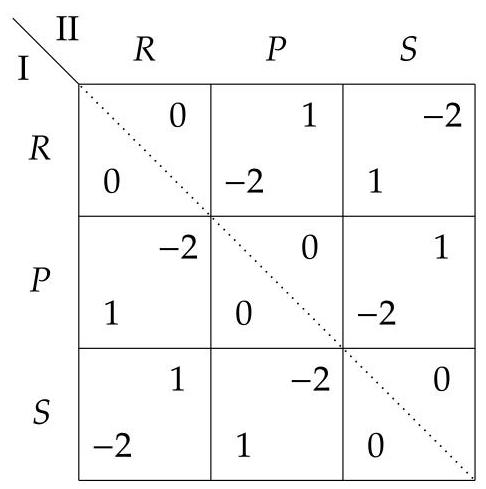
\includegraphics[width=0.3\textwidth]{images/ch12-fig05.jpg}
\end{center}
\hspace*{3em} 

(a) 找出该博弈的一个纳什均衡，并计算两个参与人在此均衡下的收益。证明当把这个纳什均衡视为相关均衡时，所有激励约束\eqref{eq:12.4}和\eqref{eq:12.5}都是紧的(即取等号)。这一事实可能足以表明该纳什均衡和相关均衡是唯一的；另一种证明方法见von Stengel and Zamir (2010，注13)。

(b) 找出该博弈的一个粗糙相关均衡，满足参与人在此均衡下的期望效用高于 (a) 中的纳什均衡。
\end{exercise}

\begin{exercise}\label{exer:12.3}
对于图~\ref{fig:12.4}中的博弈，右侧的粗略相关均衡 \(z\) 仅对策略组合 (B, M) 赋予正概率 \(a = {z}_{32}\) ，对策略组合 (M, B) 赋予正概率 \(b = {z}_{23}\) ，其他分量 \({z}_{ij}\) 均为零。找出所有可能的 \(a\) 和 \(b = 1 - a\) 的值，使得以这种方式定义的相关机制 \(z\) 构成该博弈的一个粗糙相关均衡。
\end{exercise}

\begin{exercise}\label{exer:12.4}
证明在一个有 \(N\) 个参与人且每个参与人有两种策略的博弈中，每个粗糙相关均衡都是相关均衡。
\end{exercise}

\begin{exercise}\label{exer:12.5}
证明如果 \(Y\) 是一个两状态的马尔可夫链，那么 \(Y\) 的非对角元素在其所在列中与 \(Y\) 的平稳分布 \(x\) 的概率成比例。即，如果

\[
Y = \left( \begin{array}{ll} a & b \\  c & d \end{array}\right)
\]

那么 \(\left( \begin{array}{ll} c & b \end{array}\right)  = \left( {c + b}\right) {x}^{\top }\) 。 \(x\) 何时是唯一的？请给出详细论证。
\end{exercise}
